%!TEX root = main_RECOMB.tex
\section{Results}
\label{sec:results}

\subsection{Implementation}
The software was implemented in Python2.7 using the \textit{mpmath}~\cite{mpmath} library
for  arbitrary floating point precision. The source code is freely available at \verb+https://github.com/McGill-CSB/RNApyro+.



\subsection{Error correction in 5s rRNA}

To illustrate the potential of our algorithm, we applied our techniques to identify and correct point-wise errors in RNA sequences
with conserved secondary structures. More precisely, we used \RNApyro to reconstruct 5s rRNA sequences with randomly distributed
mutations. This experiment has been designed to suggest further applications to error-corrections in pyrosequencing data.

We build our data set from the 5S rRNA multiple sequence alignment (MSA) available in the Rfam Database 11.0 (Rfam id: \texttt{RF00001}).
Since our software does not currently implement gaps (mainly because scoring indels is a challenging issue that cannot be fully addressed
in this work),  we clustered together the sequences with identical gap locations. From the $54$ MSAs without gap produced, we selected the
biggest MSA  which contains $130$ sequences (out of $712$ in the original Rfam MSA). Then, in order to avoid any bias, we used \texttt{cd-hit}
\cite{CDHIT} to remove sequences with more than 80\% of sequence similarity. This operation resulted in a data set of $45$ sequences. 

We design our benchmark using a leave-one-out strategy. We randomly picked one sequence from our data set and performed $12$ random
mutations. Our sequences have $119$ nucleotides, thus the number of mutations corresponds to an error-rate of 10\%. We repeated this operation 
$10$ times. 

To evaluate our method, we computed a ROC curve representing the performance of a classifier based on the mutational probabilities computed by
\RNApyro. We report in Table \ref{tab:benchmark} the area under the curve (AUC). More specifically, we fix a threshold $\lambda \in [0,1]$ and we
predict an error at position $i$ in sequence $\omega$ if and only if the probability $P(i,n)$ of a nucleotide $n \in \{ A,C,G,U \}$ exceed this threshold.
The set of corrections is thus $\{ n \; | \;  n \in \{ A,C,G,U \} \mbox{ and } P(i,n) > \lambda \mbox{ and }  n \neq \omega[i] \}$, where $\omega[i]$ is the
nucleotide at position $i$ in the input sequence. Then, we progressively vary $\lambda$ between $0$ and $1$ to calculate the ROC curve and the AUC.



\begin{table}
\begin{center}
\begin{tabular}{|c|c|c|c|}
\hline
& 1.0 & 0.5 & 0. \\
\hline
6 & 0.69 & 0.72 & 0.74 \\
12 & 0.80 & 0.84 & 0.84 \\
24 & 0.76 & 0.84 & 0.84 \\
\hline
\end{tabular}
\end{center}
\caption{Performance of error-correction. The row index indicates the number of mutations performed with \RNApyro, and the column index indicates
the value of the parameter $\alpha$ distributing the weights of stacking pair energies vs isostericity scores. In each cell, we report the average AUC
values over the 10 experiments.}
\label{tab:benchmark}
\end{table}


\begin{figure}
\begin{subfigure}[b]{0.3\textwidth}
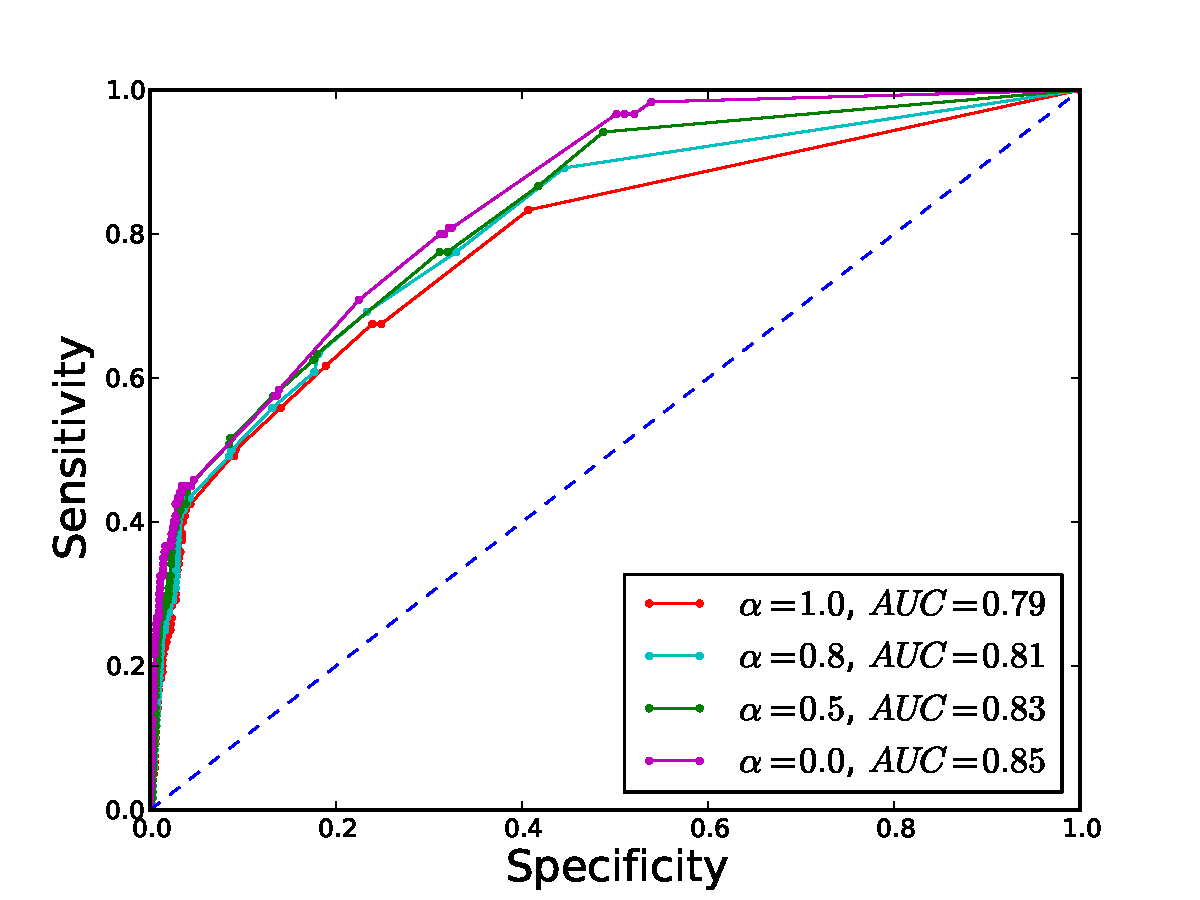
\includegraphics[width=1.2\textwidth]{figures/ROC_6.pdf}
\caption{6 mutations}
\end{subfigure}
\hfill
\begin{subfigure}[b]{0.3\textwidth}
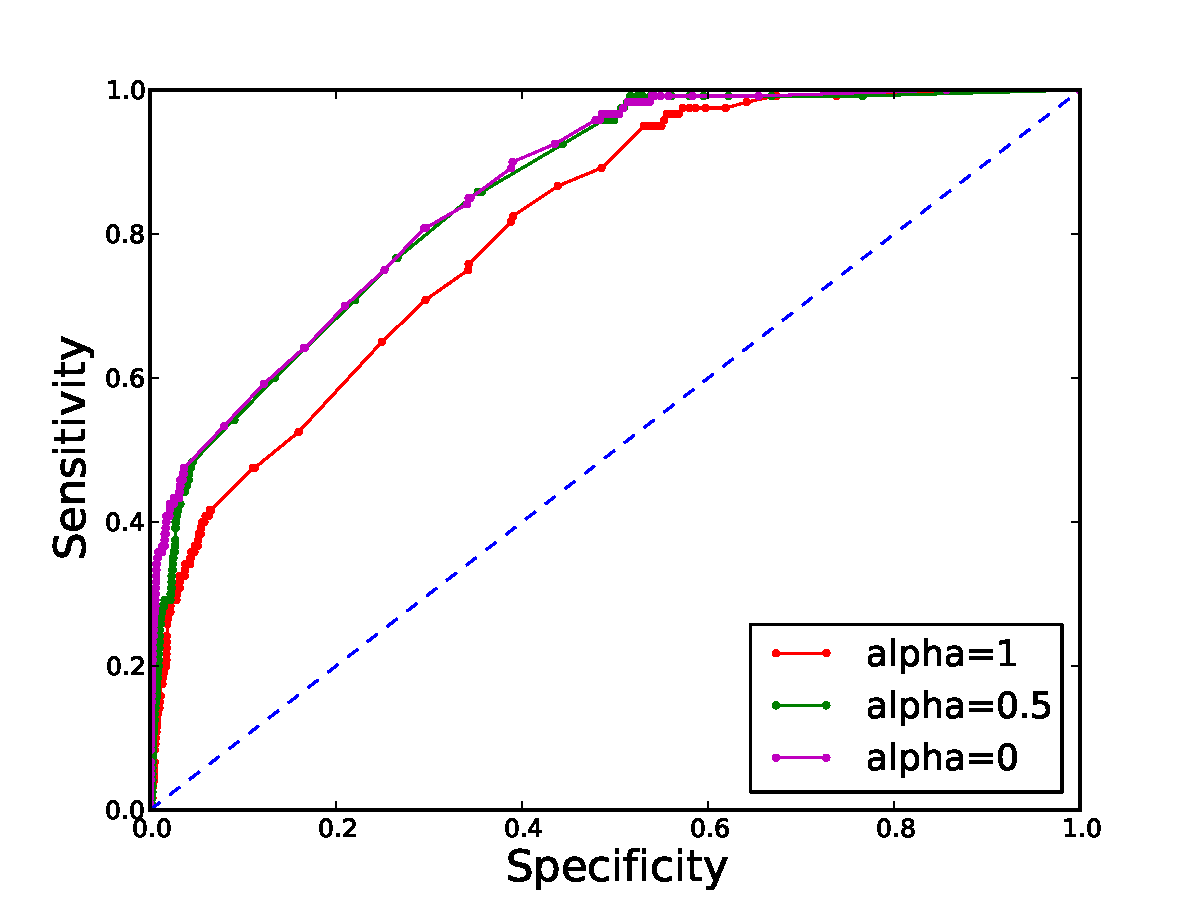
\includegraphics[width=1.2\textwidth]{figures/ROC_12.pdf}
\caption{12 mutations}
\end{subfigure}
\hfill
\begin{subfigure}[b]{0.3\textwidth}
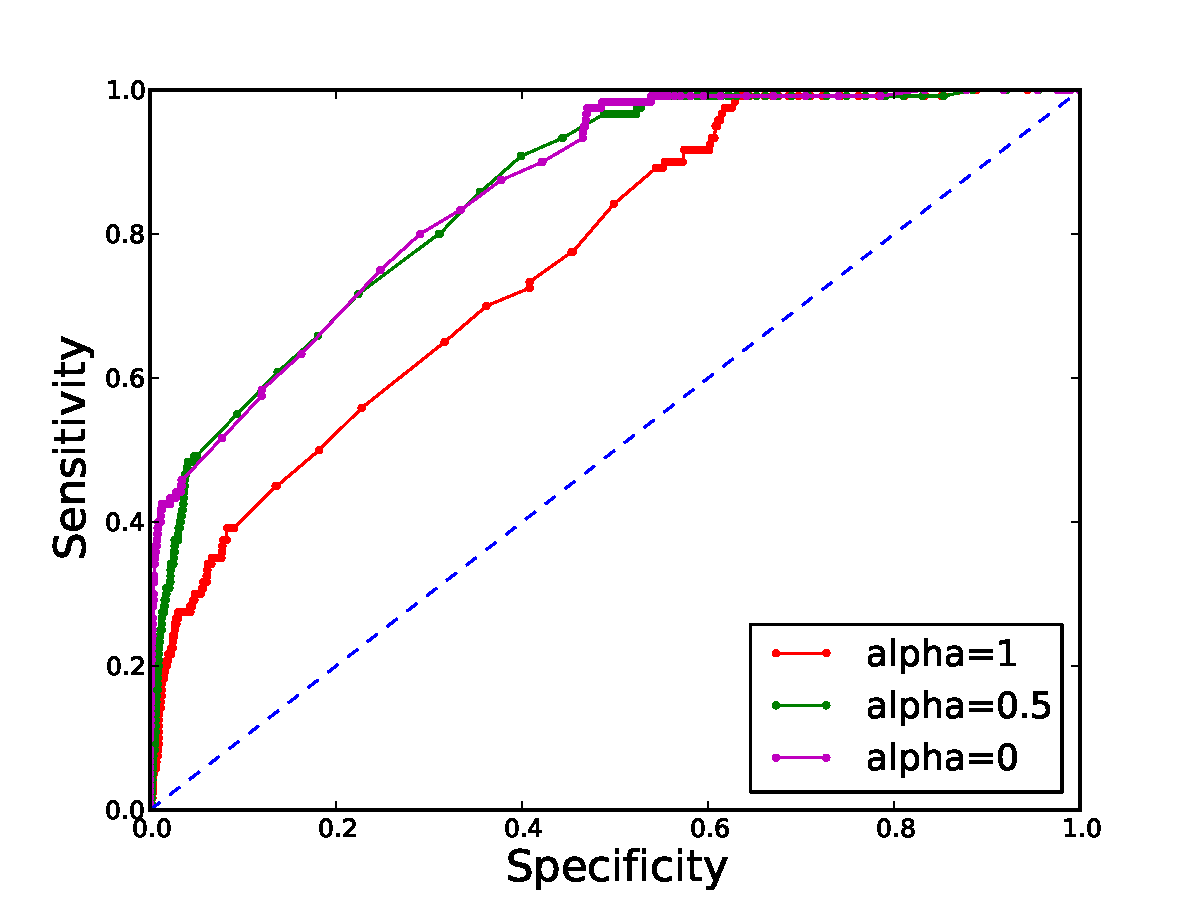
\includegraphics[width=1.2\textwidth]{figures/ROC_24.pdf}
\caption{24 mutations}
\end{subfigure}
\end{figure}




\subsection{Time}
The applications for this algorithms implies a need for efficiency
and scalability. In Table~\ref{tab:time} we
present different times needed to compute the probabilities for
 every nucleotide at every positions for a vast set of parameters. For those test
 all the sequences were generated randomly, as the target secondary structure.

\begin{table}
\begin{center}
\begin{tabular}{lccc}
$|s|$&\multicolumn{3}{c}{Number of mutations}\\\cline{2-4}
		 			  & 6   &  12  & 24\\\cline{2-4}
100  				& 35s  & 238s & 1023s\\
300  			& 135s & 594s &2460s\\\cline{2-4}
		 						& 25   & 30   &			\\\cline{2-4}
300       &      &  3950s&     \\
500         & 5400s&       &      \\
\end{tabular}
\end{center}
\caption{Time to compute all probabilities. The first column indicates the length and  the column indexes indicate the number
 of mutations. $\alpha$ is
set at $0.5$, and $\beta=1.5$ and $|\Omega|=44$.}
\label{tab:time}
\end{table}
